\documentclass[12pt,titlepage]{article}
\setlength\parindent{0pt}
\usepackage{style}

\begin{document}

\begin{enumerate}
    \item This $W$ is cut into two pieces of equal area by the straight line. The straight line intersects the right edge of the $W$ at a point. Exactly what ratio does this point split the lengths of the right edge into? 
    \begin{figure}[h]
    	\centering
    	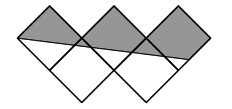
\includegraphics[scale = 1]{type2_1.png}
    \end{figure}
    \item Ezra rolls $3$ fair dice. The sum of the three numbers is equal to $n$ with probability $p_n$. What is the maximum value of $p_n$?

    \item Find the number of polynomials which satisfy $p(0) = 0$ and $p(z^2 + 1) = p(z)^2 + 1$. 

    \item Evaluate the sum
    \[
    	\frac{1}{2^2 - 1} + \frac{1}{4^2 -1} + \frac{1}{6^2-1} + ... + \frac{1}{2020^2 - 1}. 
    \]

    \item Find the last two digits of $\displaystyle \left ( \sum_{n = 1}^{2019} n! \right )^{2019}$. 

    \item There are $2019$ lockers in a gym, numbered from $1$ to $2019$, and they all start closed. There are also $2013$ students. On the first day, student $\# 1$ toggles the status of lockers $1, 2, 3, ..., 2019$. (Since they were all closed, they are now all open.) On the second day, student $\# 2$ toggles the status of lockers $2, 4, 6, ..., 2018$. On the $i$th day, student $i$ toggles the status of lockers $i, 2i, 3i, ...$ How many lockers are open after all $2019$ students have passed through?  

    \item Find the smallest integer $n$ for which there exist $n \geq 6000$ distinct pairs $(x_1, y_1), ..., (x_n, y_n)$ of positive integers with $1 \leq x_i, y_i \leq 2019$ for $i = 1, 2, ..., n$ such that for any indices $r, s \in \{1, 2, ..., n\}$ (not necessarily distinct), there exists an index $t \in \{1, 2, ..., n\}$ such that $2019$ divides $x_r + x_s - x_t$ and $y_r + y_s - y_t$. 

    \item Consider a $8 \times 8$ grid. Several of the tiles have tokens on them and there can only be one token on any tile. Call any tile \textit{Alan} if there exists an adjacent tile with a token on it. What is the minimum number of tokens needed so that all tiles of the chessboard are \textit{Alan}? \\
    (Note: tiles are considered adjacent if and only if they share a side). 
\end{enumerate}
\end{document}
